\anonsection{Условие лабораторной работы}
Требуется реализовать ПО, позволяющее генерировать алгоритмическим методом последовательность случайных чисел и проверять итоговую последовательность на случайность по любому критерию.
Также нужно добавить пользователю возможность генерировать последовательность из однозначных чисел и реализовать генерацию табличным методом.

\anonsection{Теоретическая часть}
В этом разделе будет приведено описание методов генерации последовательности случайных чисел и описан критерий проверки последовательности на случайность.

\subsection*{Виды генераторов случайных чисел}
Всего можно выделить четыре типа генераторов случайных чисел:
\begin{enumerate}
	\item \textbf{Аппаратные генераторы} используют результаты определённых физических процессов для создания требуемой последовательности. Аппаратный генератор случайных чисел состоит из источника энтропии и устройства, преобразующего значения, полученные с источника энтропии, в нужный формат.
	
	К такому типу относятся генераторы, основанные на фотоэффекте или тепловом шуме при работе полупроводникового диода. 
	На выходе получается последовательность, обладающая значительной степенью случайности, но у таких генераторов есть два недостатка: системы трудно реализовать в жизни, а процессов, позволяющие преобразовать энтропию в последовательность.
	
	\item \textbf{Алгоритмические генераторы} основаны на фиксированных алгоритмах, которые, в зависимости от некоторых физических параметров (например, содержимого ввода/вывода), выдают нужный результат. Подобные алгоритмы имеют программную реализацию и используются в коммерческом ПО.
	
	\item \textbf{Табличные генераторы} принимают на вход уже готовую последовательность, обладающую свойством случайности, после чего проводит различные манипуляции с ней (комбинирование, перемешивание), и выдают результат.
	К недостаткам этого подхода можно отнести лишнее использование памяти, предопределённость значений и ограниченность последовательности.
\end{enumerate}


\subsection*{Выбранный критерий определения случайности}
В качестве критерия был выбран критерий серий.

Пусть $l_n$ --- медиана наблюдаемых случайных величин. Каждому элементу выборки поставлен в соответствие знак ``+'' или ``-'' в зависимости от того больше он медианы или меньше. Пусть $n_1$ --- число плюсов, а $n_2$ --- число минусов. Серией называется последовательность из одинаковых знаков, ограниченная противоположными. Статистикой критерия является число серий $n$. Критическая область определяется неравенствами $n \le N_1$ и $n \ge N_2$, которые определяются из таблицы при малых значениях $n_1+n_2$. 


\begin{figure}[H]
	\centering
	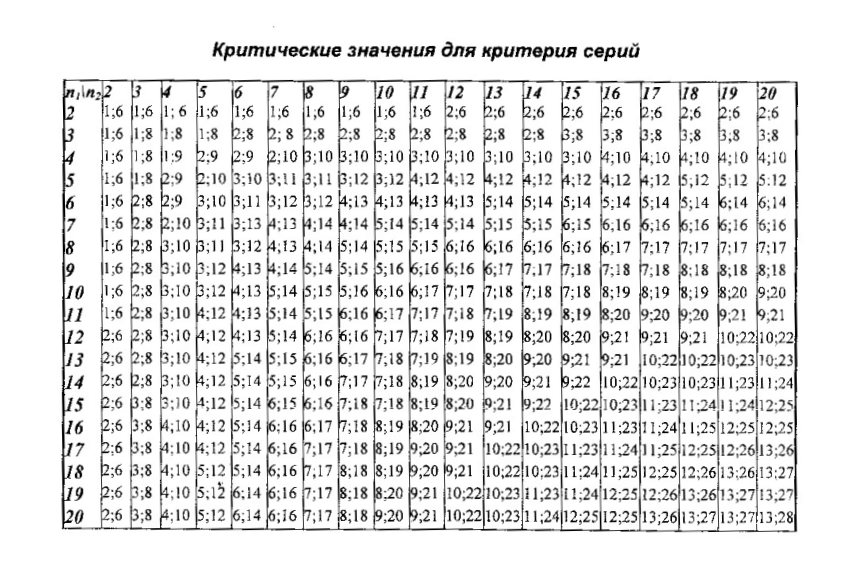
\includegraphics[width=1\linewidth]{inc/serial-table}
	\label{fig:serial-table}
\end{figure}`

Если $\max(n_1, n_2) \ge 20$, то

\[z_B=\frac{|n - \frac{2n_1n_2}{n_1+n_2} - 1| - \frac{1}{2}}{\sqrt[]{\frac{2n_1n_2(2n_1n_2-(n_1+n_2))}{(n_1+n_2)^2(n_1+n_2+1)}}} \sim N(0,1)\]
критическая область определяется неравенством 
\[z_B \le U_{\frac{\alpha}{2}} \text{	или	} z_B \ge  U_{1 - \frac{\alpha}{2}}\]

\section*{Демонстрация работы программы}

В ходе выполнения программы пользователю доступно меню, в котором он может выбрать размер последовательности, который нужно сгенерировать, уровень значимости, а также файл, если он хочет также проверить собственную последовательность.

На рисунке представлена демонстрация работы программы:

\captionsetup{justification=centering}
\begin{figure}[H]
	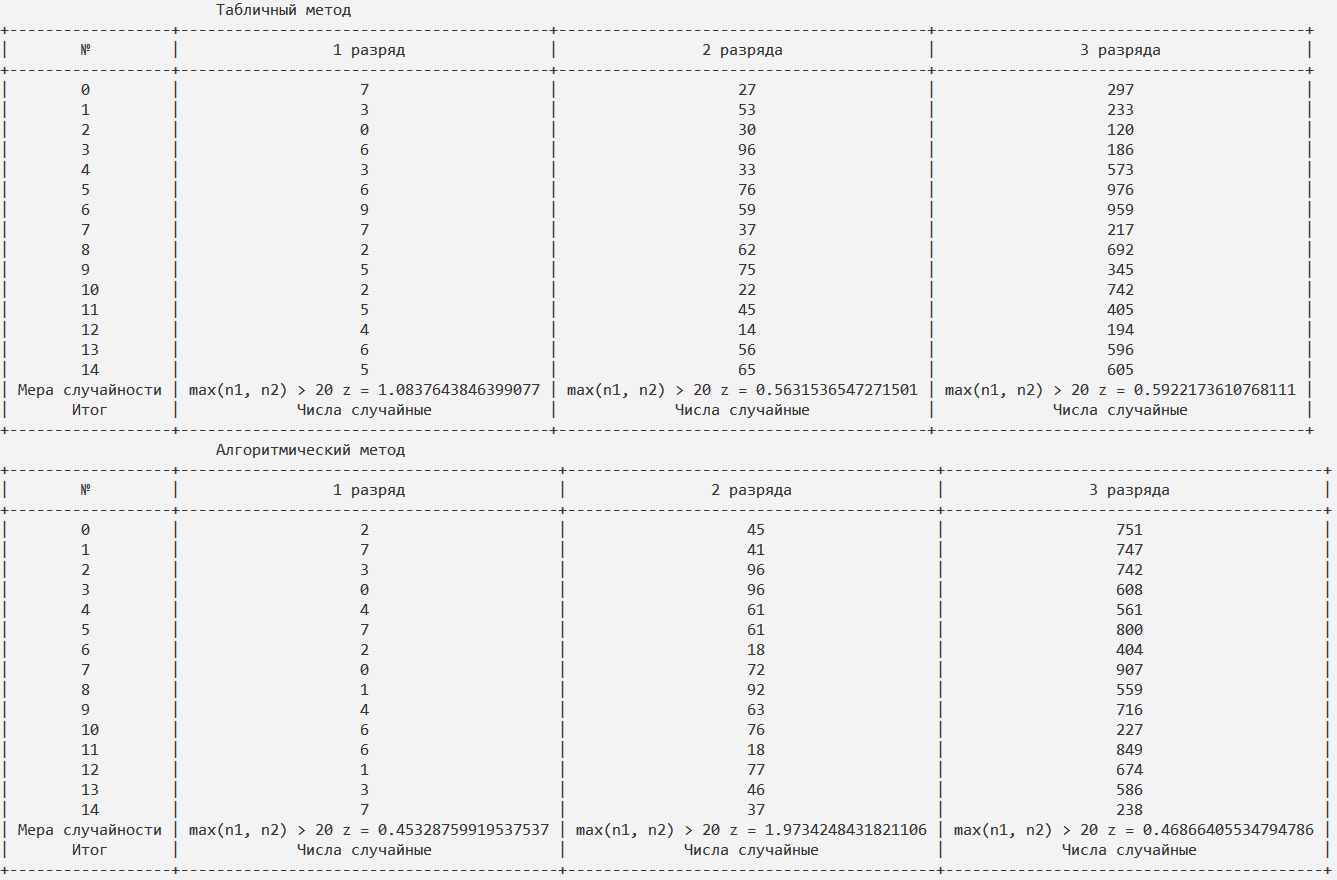
\includegraphics[width=\linewidth]{inc/demo}
	\centering
	\caption{Демонстрация работы программы}
\end{figure}


